\section{Diagram przypadków użycia}
    \subsection{Rysunek (diagram)}

    \begin{figure}[!htb]
        \centering
        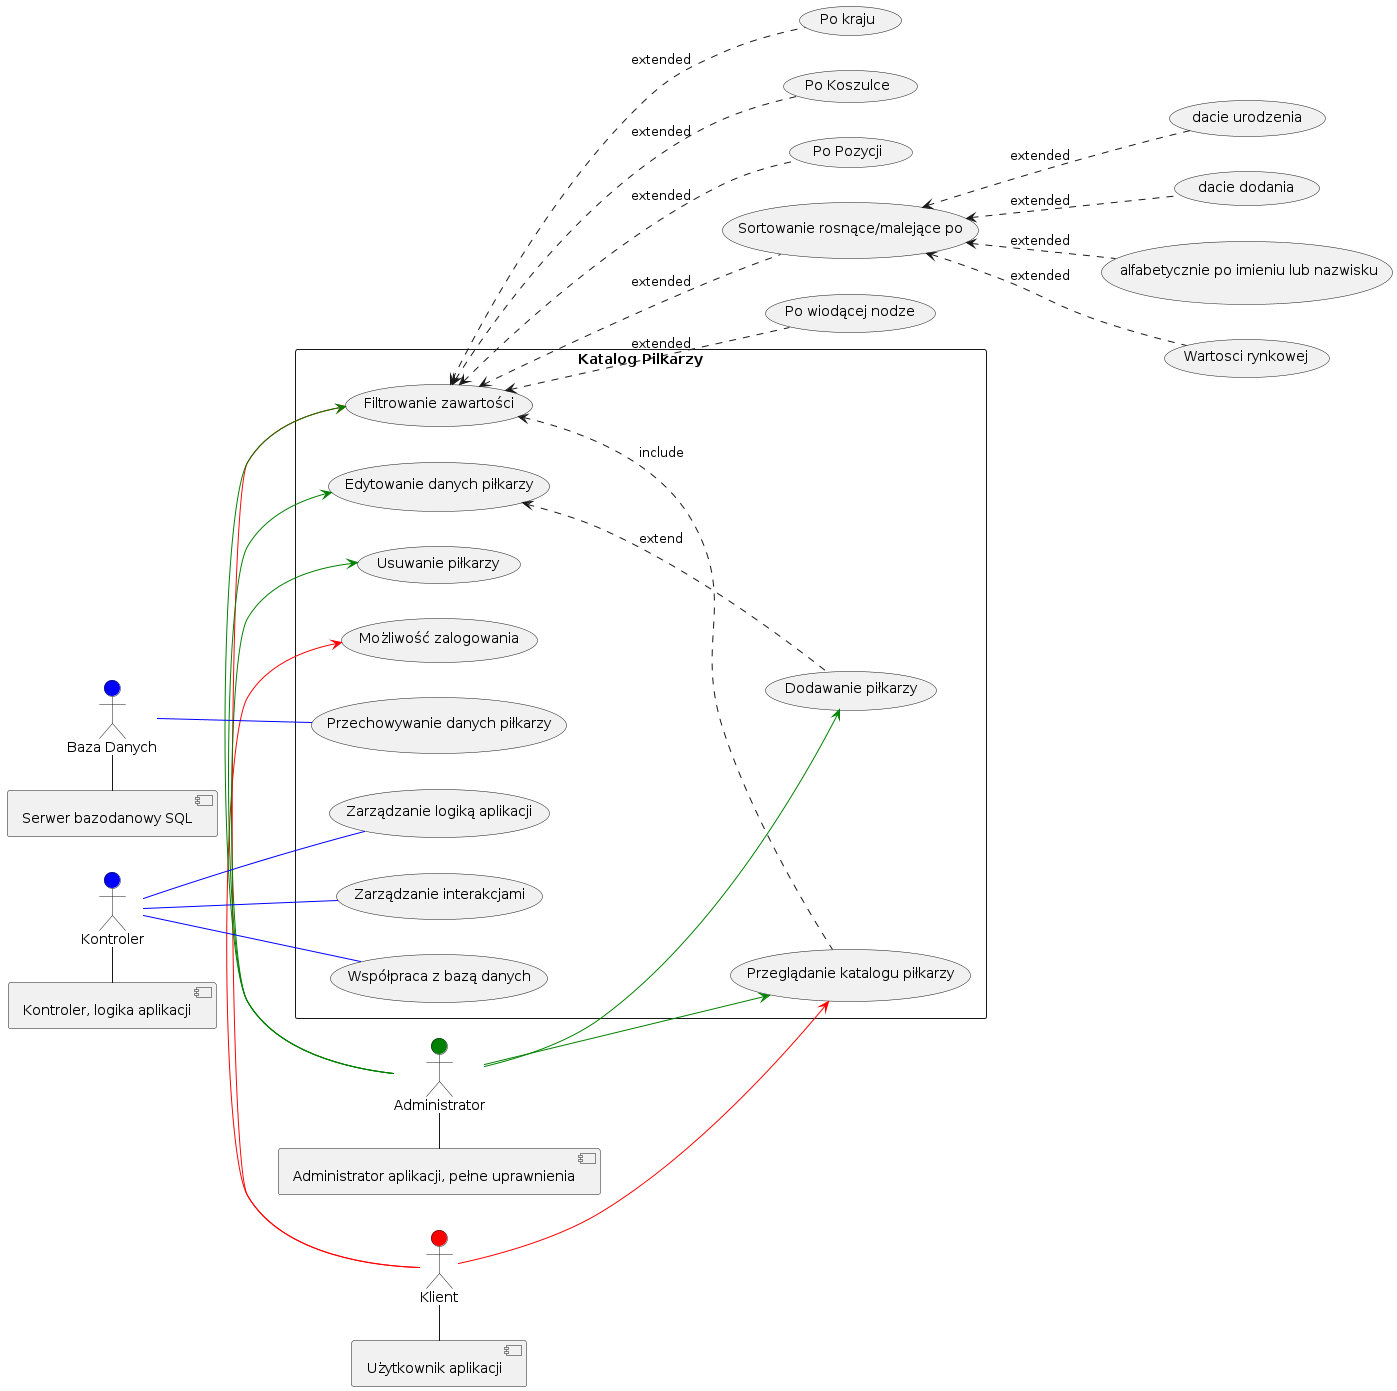
\includegraphics[width=0.9\textwidth]{diagramy/uzycia.png}
        \caption{Diagram przypadków użycia}
    \end{figure}

    \subsection{Opis}


        \textbf{Aktorami osobowymi} są: Administrator oraz Klient, są to odbiorcy aplikacji\\
        \textbf{Aktorami bezosobowymi}, abstrakcyjnymi są:
        \begin{itemize}
            \item Kontroler – reprezentuje logikę aplikacji
            \item BazaDanych – reprezentuje miejsce, gdzie informację so przechowywane
        \end{itemize}

        \textbf{Podstawowe operacje aktorów:}
        \begin{itemize}
            \item Klient -> (Przeglądanie katalogu piłkarzy)
            \item Klient -> (Filtrowanie zawartości)
            \item Klient -> (Możliwość zalogowania)
            \item Administrator -> (Przeglądanie katalogu piłkarzy)
            \item Administrator -> (Filtrowanie zawartości)
            \item Administrator -> (Dodawanie piłkarzy)
            \item Administrator -> (Edytowanie danych piłkarzy)
            \item Administrator -> (Usuwanie piłkarzy)
            \item BazaDanych -- (Przechowywanie danych piłkarzy)
            \item Kontroler -- (Zarządzanie interakcjami)
            \item Kontroler -- (Współpraca z bazą danych)
            \item Kontroler -- (Zarządzanie logiką aplikacji)
        \end{itemize}

        
        
       
       
        
        
        
        
       
        
        
        